\chapter{Objects' Alignment in Robotics.}  
 \label{chap:opt_rot}
 
 In this chapter, we are concerned with the problem of optimally aligning two vectors, a model point/shape to a ``sensed" point/shape in space \eg $\nu_1, \nu_2 \in \mathbb{R}^n$ to one another with the minimal amount of errors. There exists many methods of solving this problem. Most of them leverage clever optimization methods and we will be looking into these in this chapter. We could follow the homogeneous transformation scheme we presented in Chapter \ref{chap:intro}, but we would not have an optimal solution. A popular technique in computer geometry and computer vision is to use the iterative closest point algorithm(ICP), an algorithm by Paul Besl and Neil McKay developed out of General Motors Laboratory in the 1990's~\cite{besl1992method}. This is more appropriate for 3D tasks and it describes a generic, representation method for the accurate and computationally efficient registration of three-dimensional (3-D) shapes. The ICP algorithm always converges monotonically to the nearest local minimum of a mean-square distance metric such as an $l-2$ distance, and this convergence rate is of the order of a few iterations. An important property of the ICP algorithm is that it can register data from unfixtured rigid objects with an ideal geometrical model prior to shape inspection. So, if we want to figure out that two geometric representations are congruent, estimate the motion between them in real-time where the correspondences are not known, ICP tends to be really good for such operations.
 
 Now, suppose our dataset is not a complex geometric primitive\footnote{We shall refer to a geometric primitive as a primitive 3D shape such as a cylinder, square, prism and the likes.}, but rather a set of two vectors such that we are tasked with the problem of determining the best \textit{unconstrained transformation} between the two sets of coordinates. We can formulate the problem into a constrained optimization problem and thereafter, through clever factorization, turn the problem into a simple one of factorizing the unconstrained transformation  into a symmetric and orthogonal matrix by which we may solve for the optimal rotation and translation. The algorithm we shall be looking into will be the one that was invented in crystallography in 1976 and updated in 1978 by Wolfgang Kabsch, today dubbed the Kabsch algorithm~\cite{Kabsch1978}. Kabsch showed that a direct solution was possible, irrespective of the non-linear character of the problem.
 
 While other newer algorithms exist, these are the two popular algorithms that we shall be concerning ourselves with in this chapter.
 
 \section{Kabsch Algorithm}
 
 Suppose we have two sets of vectors $\bm{x_n}$ and $\bm{y_n}$ where $n=1,\ldots, N$, and weight $w_n$ that corresponds to each pair $\bm{x_n}$ and $\bm{y_n}$. Our goal is to find an orthogonal matrix $\cup = (u_{ij})$ which minimizes the cost function
 %
 \begin{align}
 	C = \frac{1}{2} \Sigma_n w_n \left(\cup \bm{x_n} - \bm{y_n}\right)^2 
 	\label{eq:kabsch_unconstraint}
 \end{align}
 %
 subject to 
 %
 \begin{align}
 	\sum_k u_{ki} u_{kj} - \delta_{ij} = 0
 	\label{eq:kabsch_constraint}
 \end{align}
 %
 where $\delta_{ij}$ are the elements of a unit matrix. When there is a translation, we can find the centroid of the vector sets to the origin.
 
 In order to solve the problem, we may introduce a symmetric Lagrangian matrix of multipliers, $L = (l_{ij})$ and an auxiliary function as follows
 %
 \begin{align}
 	D = \frac{1}{2} \Sigma_{i,j} l_{ij} \left(\Sigma_k u_{kl} u_{kj} - \delta_{ij}\right)
 \end{align}
 %
 so that we can form the Lagrangian, $E= C+D$. For each condition in \autoref{eq:kabsch_constraint}, we have an independent number $l_{ij}$ so that the constrained minimum of $C$ is part of the free minima of $D$. A free minimum of $D$ can occur if
 %
 \begin{align}
 	\frac{\partial E}{\partial u_{ij}} = \sum_k u_{ik} \left(\Sigma_n w_n x_{nk}x_{nj} + l_{k,j}\right) - \sum_n w_n y_{nl} x_{nj} = 0
 	\label{eq:kabsch_deri1}
 \end{align}
 %
 and 
 %
 \begin{align}
 	\frac{\partial^2 E}{\partial u_{mk} \partial u_{ij}} = \delta_{mi} \left(\Sigma_n w_n x_{nk} x_{nj} + l_{kj}\right)
 	\label{eq:kabsch_deri2}
 \end{align}
 %
 are elements of a positive definite matrix $x_{nk}$ and $y_{nk}$ are the $k$th elements of $\bm{x_n}$ and $\bm{y_n}$. Now, suppose we have a matrix $R=(r_{ij})$ and a symmetric matrix $\bm{S} = \left(s_{ij}\right)$, such that
 %
 \begin{align}
 	r_{ij} = \sum_n w_n y_{ni} x_{nj}
 \end{align}
 %
 and
 %
 \begin{align}
 	s_{ij} = \sum_n w_n x_{ni} x_{nj}.
 \end{align}
 %
 If the matrix \eqref{eq:kabsch_deri2} has $1$ along its diagonal, we must have the minimum of the Lagrangian E to mean that $S+L$ is positive definite, and \eqref{eq:kabsch_deri1} translates to 
 %
 \begin{align}
 U . \left(S+L\right) = R.
 \label{eq:pre_rot}
 \end{align}
 %
 Our goal would be to find a matrix $L$ of Lagrange multipliers so that $\cup$ is orthogonal. We can do this by multiplying both sides of \eqref{eq:pre_rot} by their transposed matrices so that we can get rid of matrix $\cup$ as follows:
 %
 \begin{align}
 	U {(S+L)}^T(S+L) &= {(S+L)}^T{U}^TU(S+L) \nonumber \\
 	&= (S+L)(S+L) = {R}^TR.
 \end{align}
 %
 Now, we know that ${R}^TR$ is a symmetric positive definite matrix so that we can find the eigenvalues $\lambda_k$ and eigenvectors $\bm{v}_k$ using standard procedures \eg single value decomposition. Thus, since $S+L$ is symmetric and positive definite, it must have normalized eigenvectors, $\bm{v}_k$ and positive eigenvalues $\sqrt{\lambda_k}$  so that the Lagrange multipliers are
 %
 \begin{align}
 	l_{ij} = \Sigma_k \sqrt{\lambda_k}; \qquad \qquad \bm{v}_{ki} \bm{v}_{ki} - s_{ij}
 \end{align}
 %
 where $\bm{v}_{ki}$ signifies the $i$th component of $\bm{v}_k$ and the effect of the orthogonal matrix $U$ on these eigenvectors $\bm{a}_k$ is determined from \eqref{eq:pre_rot} which defines the unit vectors $\bm{q}_k$ as 
 %
 \begin{align}
 	\bm{q}_k = U . \bm{v}_k = \frac{1}{\sqrt{\lambda_k}} U (S+L) \bm{v}_k = \frac{1}{\sqrt{\lambda_k}} R \bm{v}_k.
 \end{align}
 
 The solution to find the constraint minimum of the minimum of the proposed cost function in \eqref{eq:kabsch_unconstraint} is then given by,
 %
 \begin{tcolorbox}[title=Kabsch's Optimal Rotation]
 	\begin{align}
 		u_{ij} = \Sigma_k b_{kl} a_{kj}.
 	\end{align}
 \end{tcolorbox}

\subsection{Examples}
%
There are clever ways of solving the optimal rotation between two vectors.

There is a jupyter notebook at the following  link: \href{https://colab.research.google.com/drive/1DL_Hq-Bp-pQuQyR6nDHnzwxIqhj4_Obq}{Kabsch Algorithm and Implementation}. For your convenience, it is included as a pdf file below.

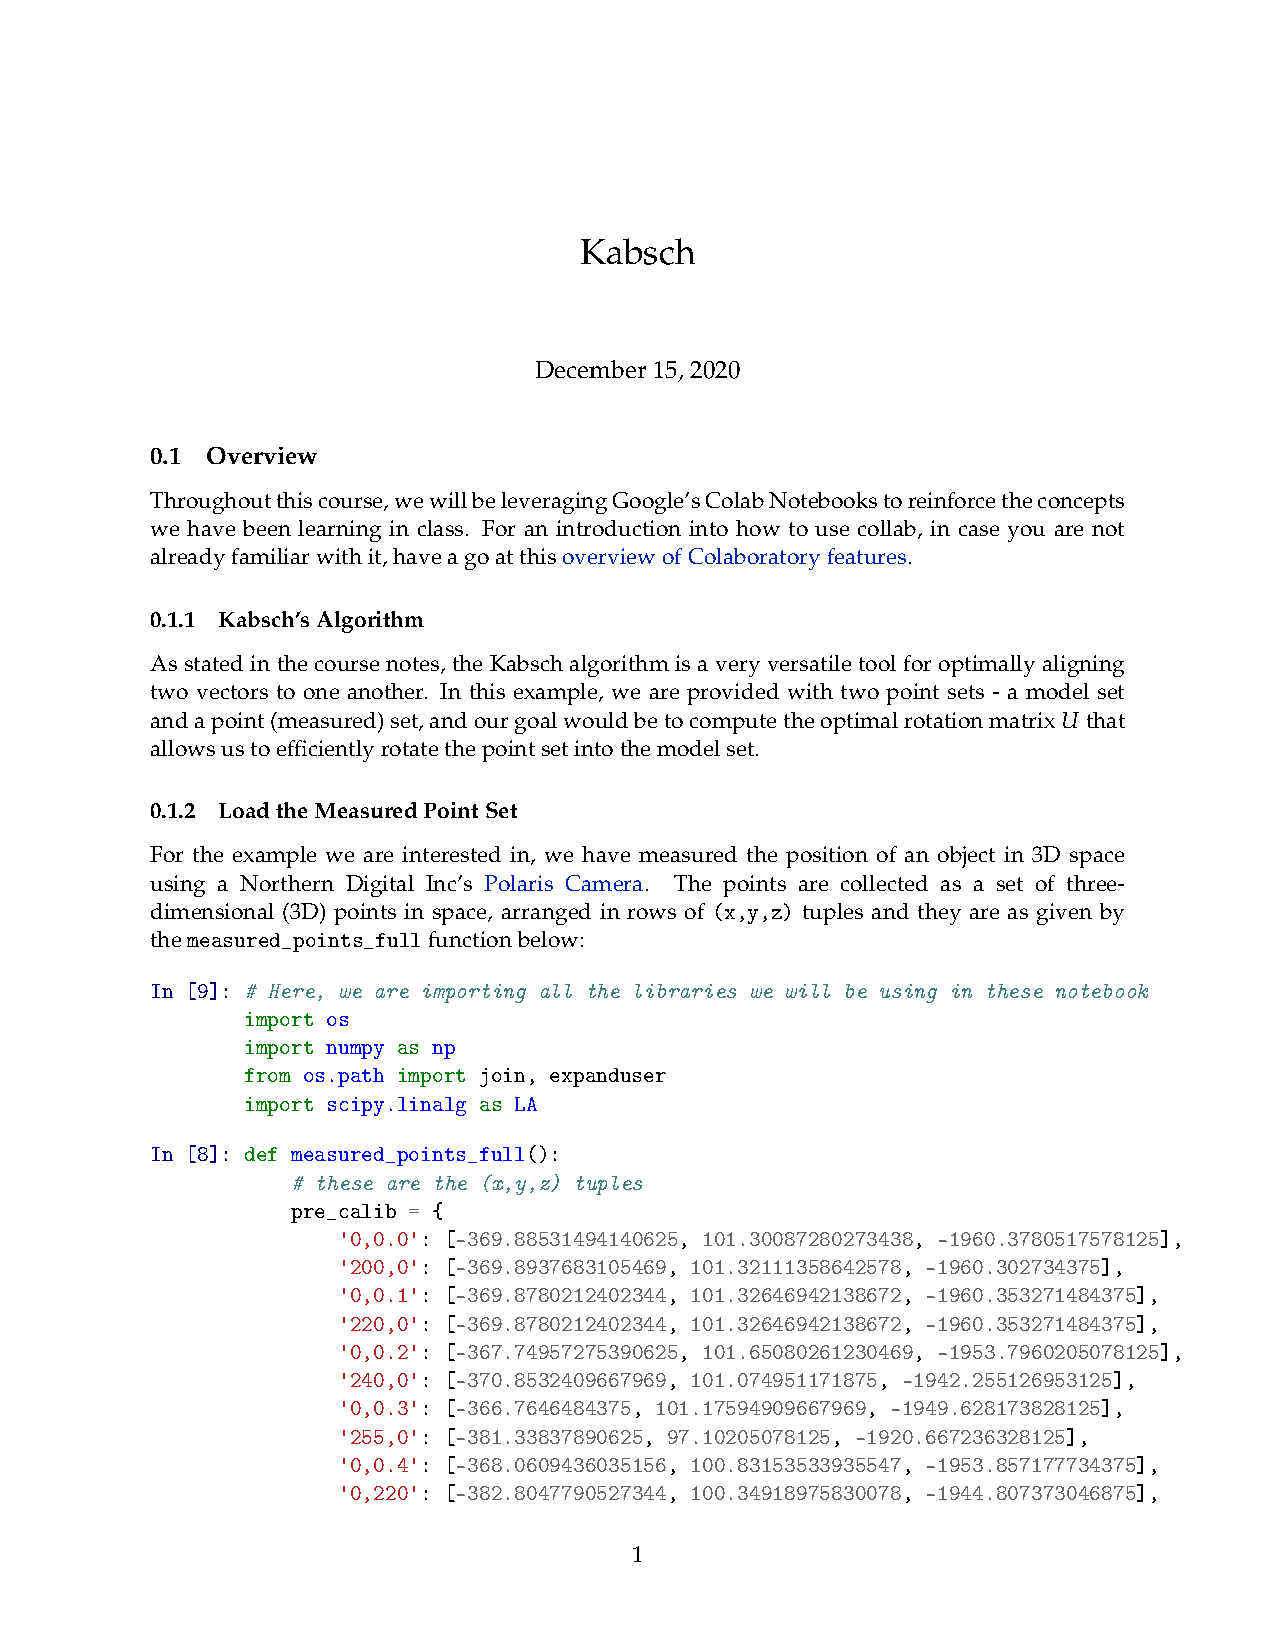
\includepdf[pages=1-]{Kabsch.pdf}

